%% Template for MLP Coursework 1 / 16 October 2017 

%% Based on  LaTeX template for ICML 2017 - example_paper.tex at 
%%  https://2017.icml.cc/Conferences/2017/StyleAuthorInstructions

\documentclass{article}

\usepackage[T1]{fontenc}
\usepackage{amssymb,amsmath}
\usepackage{txfonts}
\usepackage{microtype}

% For figures
\usepackage{graphicx}
\usepackage{svg}
\usepackage{subfigure}

% For citations
\usepackage{natbib}

% For algorithms
\usepackage{algorithm}
\usepackage{algorithmic}

% the hyperref package is used to produce hyperlinks in the
% resulting PDF.  If this breaks your system, please commend out the
% following usepackage line and replace \usepackage{mlp2017} with
% \usepackage[nohyperref]{mlp2017} below.
\usepackage{hyperref}
\usepackage{url}
\urlstyle{same}

% Packages hyperref and algorithmic misbehave sometimes.  We can fix
% this with the following command.
\newcommand{\theHalgorithm}{\arabic{algorithm}}


% Set up MLP coursework style (based on ICML style)
\usepackage{mlp2017}
\mlptitlerunning{MLP Coursework 1 (\studentNumber)}
\bibliographystyle{icml2017}


\DeclareMathOperator{\softmax}{softmax}
\DeclareMathOperator{\sigmoid}{sigmoid}
\DeclareMathOperator{\sgn}{sgn}
\DeclareMathOperator{\relu}{relu}
\DeclareMathOperator{\lrelu}{lrelu}
\DeclareMathOperator{\elu}{elu}
\DeclareMathOperator{\selu}{selu}
\DeclareMathOperator{\maxout}{maxout}

%% You probably do not need to change anything above this comment

%% REPLACE this with your student number
\def\studentNumber{s1784849}

\begin{document} 

\twocolumn[
\mlptitle{MLP Coursework 1: Activation Functions}

\centerline{\studentNumber}

\vskip 7mm
]

\begin{abstract} 
The problem domain considered within this report pertains to the use of various activation functions within deep neural networks. Specifically, the effect that leaky rectified linear units (LReLUs), exponential linear units (ELUs) and scaled exponential linear units (SELUs) have on the error and accuracy of deep neural network models and how these functions compare to a baseline ReLU and sigmoid function. Within the latter half of this report, an investigation into the effect of varying the number of hidden layers within neural nets is presented. Fully connected neural networks, initially with two hidden layers, then later spanning up to six layers were used. It was found that ReLU variant activation functions consistently outperformed standard sigmoid units, but there was not much variation in performance between ReLU variants for this particular problem domain\footnote{Classifying handwritten digits within the MNIST dataset.}. Whilst it was concluded that fewer layers increased the speed of convergence for this particular problem, the accuracy still reached the same level regardless of the number of layers utilised within the outlined neural network architecture.
\end{abstract} 

\section{Introduction}
\label{sec:intro}

As neural networks have become become increasingly popular over the last decade\citep{bengio2012practical} it has become important to investigate and understand the effects popular activation functions have on the training process, and how different activation functions can be used to achieve state of the art level performance on well understood research problems. Furthermore, the emergence of deep learning\citep{hinton2006fast}\citep{bengio2007greedy} has provided ample motivation for investigating the effects of employing many hidden layers within neural network architectures.

This report provides investigations into two variable aspects of neural networks that effect the potential accuracy and error achieved by these models. Initially, before any investigations are presented, an introduction to the set of activation functions that are employed by neural networks utilised within this report is provided. An experimental comparison of these activation functions is given, along with a sensitivity analysis that provides tuning for the hyper parameter usually labelled as the step size (or learning rate)\citep{jacobs1988increased}. In addition, an investigation into varying the depth of a neural network is presented and follow up conclusions about the effects this has on the potential accuracy attained by the networks is proposed.

The neural networks used for the experiments within this report are trained on the MNIST dataset. The training set is made up of 50,000 examples and the test set (which the validation examples are drawn from) is of length 10,000.

The fundamental research questions this report aims to address are outlined below.

\begin{itemize}
  \item Two hidden layer network: what is an optimal setting for the hyper parameter known as the step size (or learning rate) on the given activation functions?
  \item Two hidden layer network: which activation function provides the fastest rate of convergence towards a minimum error and maximum accuracy?
  \item Two hidden layer network: which activation functions provides the highest ceiling with regards to potential accuracy that can be acquired?
  \item N-hidden layer network: how does varying the number of hidden layers within our neural network architecture affect the overall model accuracy?
\end{itemize}

\section{Activation functions}
\label{sec:actfn}
The activation functions utilised within this report are leaky rectified linear units, exponential linear units\citep{clevert2015fast} and scaled exponential linear units\citep{klambauer2017self}. Comparisons against one another, in addition to baseline rectified linear units and sigmoid units will be presented in the next section. This section provides an introduction the aforementioned activation functions.

\subsection{Sigmoid}

Within this report a standard sigmoid function is used to provide a simple baseline to compare other activation functions to. The sigmoid activation function is defined as the following:

\begin{equation}
  \sigma(x) = \frac{1}{1+e^{-x}}
\end{equation}
With gradient:
\begin{equation}
  \frac{d}{dx} \sigma(x) = \sigma(x) \times (1-\sigma(x)).
\end{equation}

\subsection{Rectified Linear Unit}

The ReLU activation function was proposed as an alternative to the sigmoid function due to it's ability to solve the vanishing gradient problem\citep{nair2010rectified}. These units are defined as follows:

\begin{equation}
  \relu(x) = \max(0, x) ,
\end{equation}
With gradient:
\begin{equation}
  \frac{d}{dx} \relu(x) =
     \begin{cases} 
      0      & \quad \text{if } x \leq  0 \\
      1       & \quad \text{if } x > 0 .
    \end{cases} 
\end{equation}

\subsection{Leaky Rectified Linear Unit}

Although the ReLU activation function helps protect against vanishing gradients during training, it introduces other problems that must be addressed. One such problem is the introduction of dying ReLU’s, where the function will output zero in the scenario where the weighted sum of the inputs is negative. Once the unit is in this state, it’s capability for learning ceases as the gradient of any negative input results in zero, which leads to the weight updates equating to zero. LReLUs (or parameterised ReLUs - PReLUs)\citep{he2015delving} attempt to mitigate this by introducing a non-zero gradient, in the case of LReLU the hyper parameter, alpha, is typically set to 0.01. In the case of PReLU, alpha is a parameter that should be selected or tuned. LReLU is defined as the following:

\begin{equation}
  \lrelu(x) = 
    \begin{cases}
      \alpha x      & \quad \text{if } x \leq  0 \\
      x       & \quad \text{if } x > 0 .
    \end{cases}
\end{equation} 
With gradient:
\begin{equation}
  \frac{d}{dx} \lrelu(x) =
     \begin{cases}
      \alpha      & \quad \text{if } x \leq  0 \\
      1       & \quad \text{if } x > 0 .
    \end{cases} 
\end{equation}

\subsection{Exponential Linear Unit}

ELUs provide similar functionality to LReLUs and PReLUs, but aim to increase learning speed in order to reach higher classification accuracies\citep{clevert2015fast}. The ELU activation function is defined as:

\begin{equation}
  \elu(x) = 
  \begin{cases} 
    \alpha (e^{x} - 1)      & \quad \text{if } x \leq  0 \\
    x       & \quad \text{if } x > 0 .
  \end{cases}
\end{equation} 
which has the gradient:
\begin{equation}
  \frac{d}{dx} \elu(x) =
     \begin{cases} 
      \elu(x) + \alpha      & \quad \text{if } x \leq  0 \\
      1       & \quad \text{if } x > 0 .
    \end{cases} 
\end{equation}

\subsection{Scaled Exponential Linear Unit}

The SELU\citep{klambauer2017self} activation function is a variation on ELU that is defined by:

\begin{equation}
  \selu(x) = \lambda 
  \begin{cases} 
    \alpha (e^{x} - \alpha)      & \quad \text{if } x \leq  0 \\
    x       & \quad \text{if } x > 0 .
  \end{cases}
\end{equation} 
which has the gradient:
\begin{equation}
  \frac{d}{dx} \selu(x) = \lambda
     \begin{cases} 
      \alpha (e^{x})      & \quad \text{if } x \leq  0 \\
      \lambda       & \quad \text{if } x > 0 .
    \end{cases} 
\end{equation}

\section{Experimental comparison of activation functions}
\label{sec:actexpts}

The neural network model used within the initial experiment that compares activations functions was trained using 2 hidden layers, each containing 100 units. A soft-max layer was applied to the output which contained 10 units in order to classify digits from the MNIST dataset from 0 to 9. A batch size of 50 and stats interval\footnote{The interval at which statistics are recorded across the experiment, measured in epochs.} of 1 was used across all experiments.

Throughout the experiments the sigmoid and ReLU activation functions were used as baselines to compare with the performance of the other activation functions. However, it is shown in figure ~\ref{fig:sigmoid-vs-relu} that any ReLU variant function\footnote{ReLU variant functions reference ReLU, LReLU, ELU and SELU in this report.} consistently outperforms a standard sigmoid function\footnote{By standard sigmoid, this report is referring to the function described within the second section, as a tunable sigmoid may perform better.}. For this reason, the sigmoid baseline is only shown in selected figures and tables presented within this report.

\begin{figure}[tb]
\vskip 5mm
\begin{center}
%\centerline{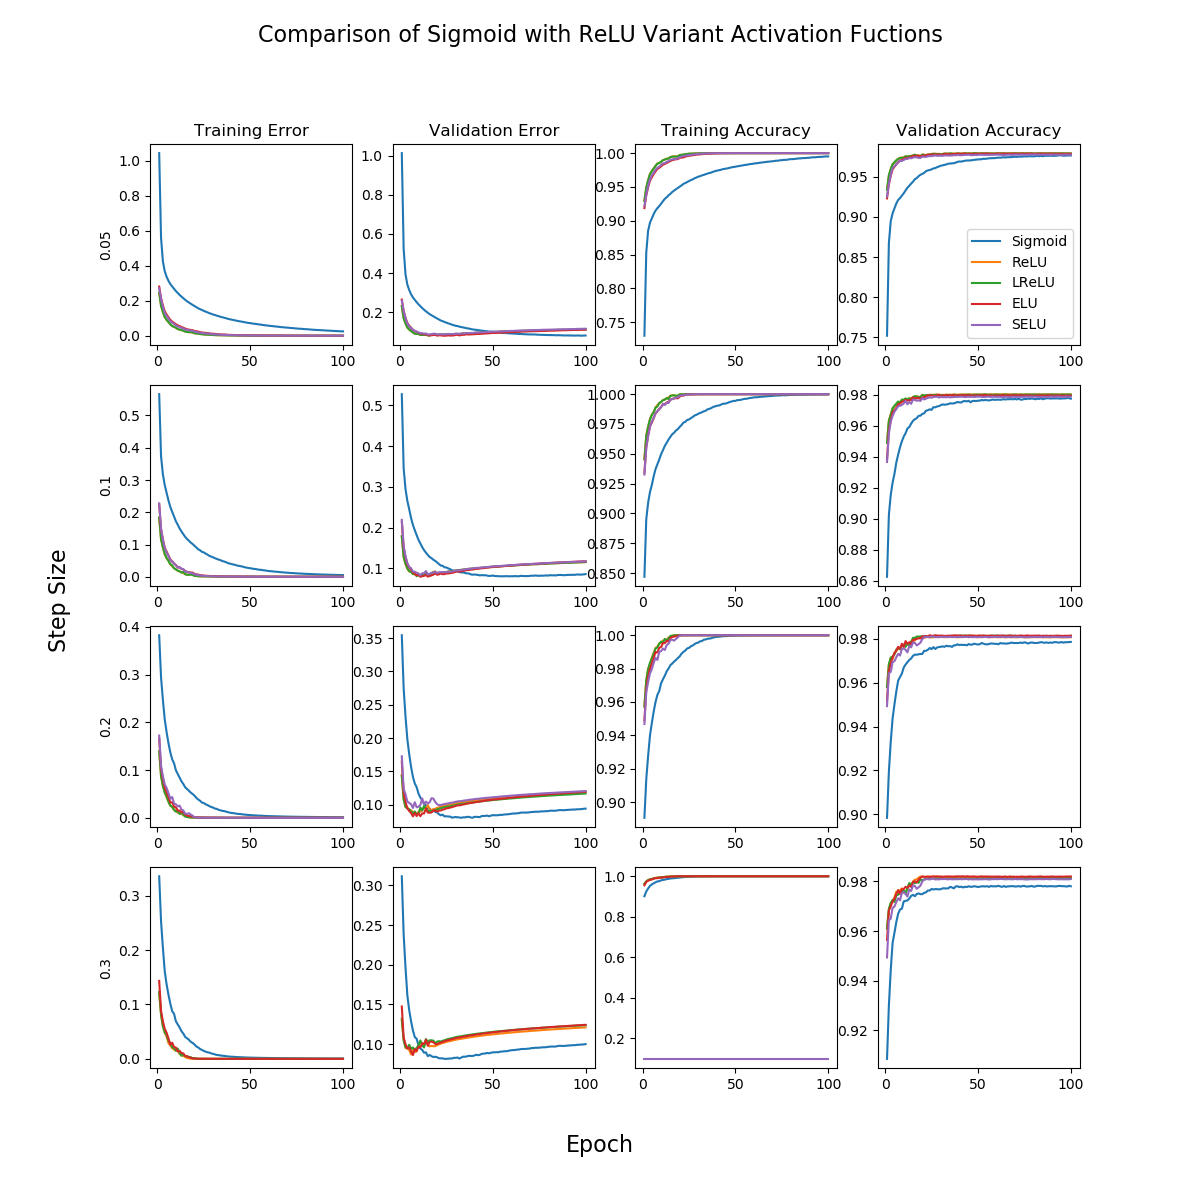
\includegraphics[width=\columnwidth]{sigmoid_vs_relu}}
\centerline{\includesvg[width=\columnwidth]{sigmoid_vs_relu}}
\caption{Training and validation error, with training and validation accuracy plotted agaisnt each epoch for step sizes: 0.05, 0.1, 0.2 and 0.5.}
\label{fig:sigmoid-vs-relu}
\end{center}
\vskip -5mm
\end{figure} 

It is shown that although ReLU variant functions consistently outperform a sigmoid baseline, there are occurrences of overfitting the test set when measuring error on the validation set. This is conveyed in figure ~\ref{fig:sigmoid-vs-relu} within the validation error column. The sigmoid line that is plotted (marked in blue) eventually crosses over the ReLU variant function lines, demonstrating that the ReLU variant functions are more sensitive to overtraining. This suggests that employing a technique such as early stoping is particularly important for these activation functions. For this reason measurements in error presented within tables throughout this report will typically be taken within 20 to 40 epochs after the experiment starts, this will be explicitly stated.

In order to find an appropriate value for the step size a sensitivity analysis was performed. The values 0.05, 0.1, 0.2 and 0.3 were used evaluate the performance of the network. In order to gauge a more reliable value for the step size, the experiments were repeated a total of five times\footnote{Ideally, experiments of this nature should be performed more than five times in order find a more reliable value for any particular hyperparameter, in this instance the experiments were repeated five times due to time constraining factors.} and the mean value for error and accuracy was taken across all of these experiments for each epoch. The following seeds were used for each experiment:

\begin{itemize}
  \item 6102016
  \item 1237878
  \item 2673679
  \item 8978283
  \item 5627351
\end{itemize}

\begin{figure}[tb]
\vskip 5mm
\begin{center}
%\centerline{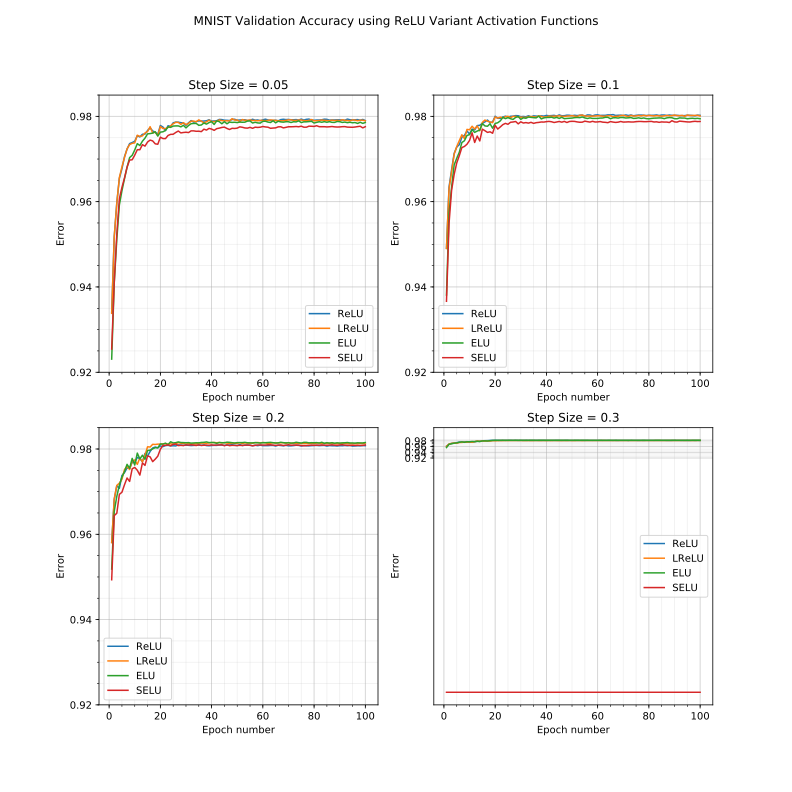
\includegraphics[width=\columnwidth]{validation_acc_sens_analysis_svg}}
\centerline{\includesvg[width=\columnwidth]{validation_acc_sens_analysis_svg}}
\caption{Validation accuracy for various step sizes (sensitivity analysis).}
\label{fig:sens-analysis-val-acc}
\end{center}
\vskip -5mm
\end{figure}

\begin{table}[tb]
\vskip 3mm
\begin{center}
\begin{small}
\begin{sc}
\begin{tabular}{lcccr}
\hline
\abovespace\belowspace
Function & Step Size & Validation Error (15 epochs) \\
\hline
\abovespace
ReLU    & 0.2& 0.094 \\
LReLU & 0.2& 0.090 \\
ELU    & 0.2& 0.088 \\
\belowspace
SELU    & 0.2& 0.101 \\
\hline
\end{tabular}
\end{sc}
\end{small}
\caption{Validation accuracies for a 2 hidden layer neural net using 
various activation functions on the MNIST dataset.}
\label{tab:MNIST-table}
\end{center}
\vskip -3mm
\end{table}

A value of 0.2 was chosen for the step size because this value provided the highest ceiling with regards to the level of accuracy that could be reached, see figure ~\ref{fig:sens-analysis-val-acc} and table 1.

\begin{figure}[tb]
\vskip 5mm
\begin{center}
%\centerline{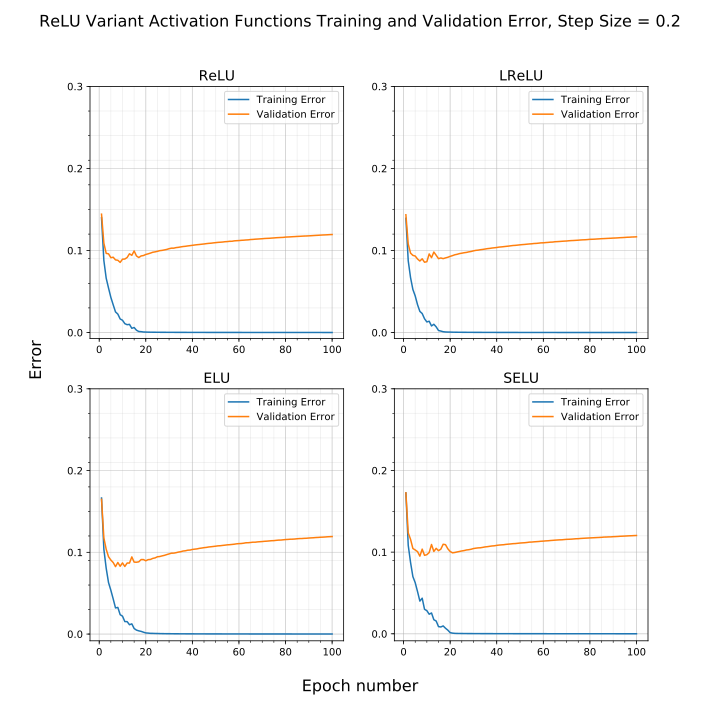
\includegraphics[width=\columnwidth]{02_relu_variants_error_svg}}
\centerline{\includesvg[width=\columnwidth]{02_relu_variants_error_svg}}
\caption{ReLU, LReLU, ELU and SELU errors plotted against each epoch.}
\label{fig:relu-variants-error}
\end{center}
\vskip -5mm
\end{figure}

\begin{figure}[tb]
\vskip 5mm
\begin{center}
%\centerline{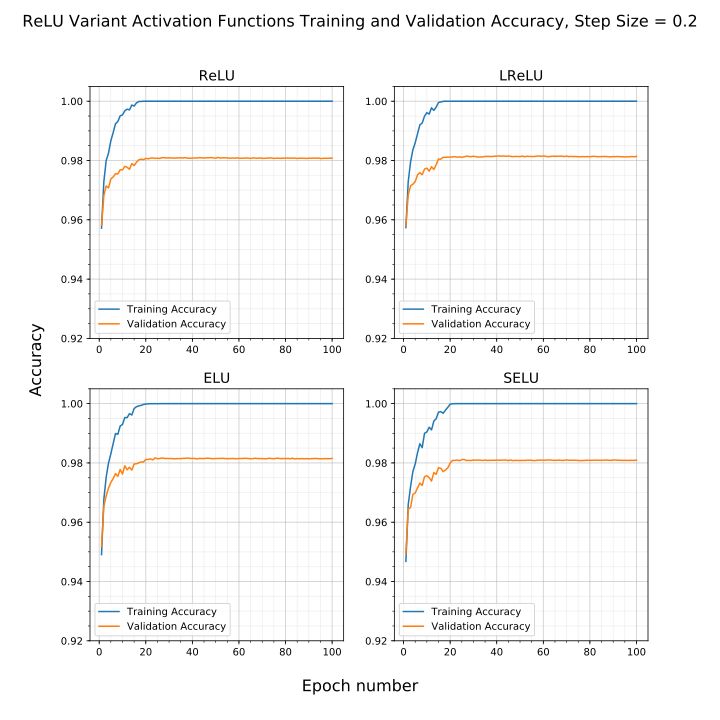
\includegraphics[width=\columnwidth]{02_relu_variants_accuracy_svg}}
\centerline{\includesvg[width=\columnwidth]{02_relu_variants_accuracy_svg}}
\caption{ReLU, LReLU, ELU and SELU accuracy plotted against each epoch.}
\label{fig:relu-variants-accuracy}
\end{center}
\vskip -5mm
\end{figure}

Figure ~\ref{fig:02_relu_variants_error_svg} shows the training and validation error, and figure ~\ref{02_relu_variants_accuracy_svg} presents the validation accuracy of all four ReLU variant functions.

\section{Deep neural network experiments}
\label{sec:dnnexpts}

\begin{figure}[tb]
\vskip 5mm
\begin{center}
%\centerline{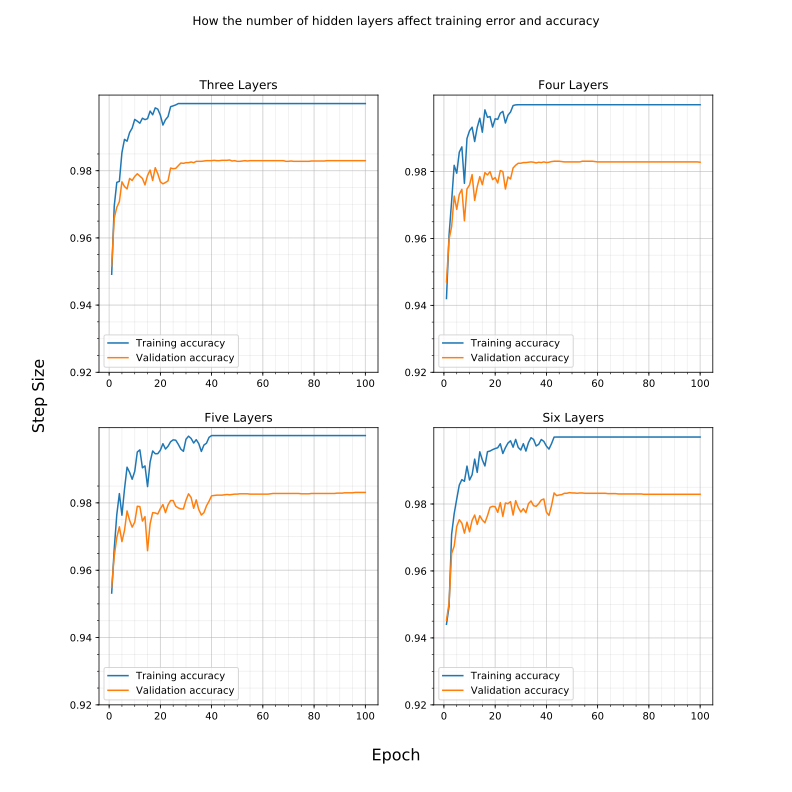
\includegraphics[width=\columnwidth]{hidden_layers_affects_svg}}
\centerline{\includesvg[width=\columnwidth]{hidden_layers_affects_svg}}
\caption{Relationship between the number of layers within a deep neural network architecture and the training and validation accuracy.}
\label{fig:dnn-accuracy}
\end{center}
\vskip -5mm
\end{figure}

Through varying the number of hidden layers within our neural network architecture (ranging between three and six hidden layers), it is possible to plot the training accuracy and validation accuracy for each layer increment. The learning rate was kept at a value of 0.2 and the ELU activation function was chosen, as it provided the best performance in the previous experiment. It was found that the accuracy generally levels out to the same point regardless of the number of layers. However, it is shown in figure ~\ref{fig:dnn-accuracy} that the more hidden layers that are used, the longer the time to convergence. The behaviour of a deeper network appears similar to initially increasing the step size.

\section{Conclusions}
\label{sec:concl}

Despite the many experiments ran in order to produce this report, the experimental results do not provide a clear narrative. It was expected that the ReLU variant activation functions would outperform the standard sigmoid function, which was indeed the case. However, the performance of each ReLU variant function did not differ much between one another for this particular problem, using this particular data (MNIST character recognition). It was expected that there would be a more noticeable difference within the result set for the performance of each function. 

Nevertheless, it was shown that the optimal learning rate for this particular problem lies within the region of 0.1 and 0.2. In addition, the ReLU variant activation functions consistently outperform a standard sigmoid function with regards to speed of convergence, however the ReLU variant functions are particularly sensitive to overtraining, indicating that early stopping is important when implementing these activation functions. Although the variation between ReLU, LReLU, ELU and SELU is almost negligible, LReLU performed the best with respect to fastest convergence, whereas ELU provided the best performance with respect to minimum error and maximum accuracy.

It was found that additional hidden layers within the outlined network architecture do not provide any additional boost in performance (specifically accuracy) for the particular problem this report aims to address. In addition, it has been shown to slow down the rate of convergence. Whilst it may appear advantageous to use fewer layers (two or three instead of five or six), it is advised to consider the complexity of the function to be approximated before considering whether or not to use additional layers. In this instance, it did not appear necessary, but deep neural networks have provided significant benefits to other problems in the past\citep{krizhevsky2012imagenet}\footnote{Different (and more complex) network architectures are typically used in other papers and reports, for example the use of convolutional layers, pooling layers, etc.}.

\subsection{Future Work}

An investigation into the modification of weight initialisation methods was going to be included within this report, but time constraining factors means that it is likely to appear within future work.

\newpage

\bibliography{example-refs}

\end{document}